\subsubsection{Genericity of MCTS Algorithm}

One of the advantages of the MCTS algorithm is its genericity. In fact it can be applied to a lot of games. In order to keep this genericity, we thought about two methods.

The first one is General Game Playing\cite{General_Game_Playing}, a formal language which allows programs to create a model given the game formal rules. However, the problem of this approach is that even if it makes it possible to play unknown games, it prevents the use of efficient heuristics to improve the algorithm.
That is why we chose another way which consists in exploiting the properties of the MCTS algorithm. 
With this solution, the algorithm does not need to know the rules, only the moves. With this in mind we created an interface for the game which defines the methods that the MCTS algorithm requires. In other words our algorithm is compatible with all the two-players games implemented with this interface.

Only the following fonctions are required : 
\begin{itemize}[nolistsep]
\item return all the possible moves given position
\item play a random move
\item play a chosen move 
\item play random moves until the end of the game
\item return whether the game is not finished or who won
\end{itemize}

\subsubsection{Branching factor}

The main game of our algorithm is Arimaa. Therefore we will be able to specialize our algorithm for it in order to improve its efficiency. The main problem is the branching factor\footnote{In a tree, the branching factor is the number of children at each node.} of the Arimaa game which average is 17 281 and reaches about 22 000 after 10 moves\cite{branchin_factor}.

\begin{center}
	\begin{tabular}{ | c | c |}
		\hline Game & Average number of possible moves \\ \hline
		\hline  
		Othello & 8\\
		\hline  
		Chess & 35\\
		\hline  
		Game of Go & 250\\
		\hline
		Arimaa & 17 281\\
		\hline
	\end{tabular}
\end{center}

The branching factor of a game is important because it increases greatly the space that has to be explored to guess what will happend multiple moves ahead. In chess after 4 moves, the number of positions evaluated are about 35\textsuperscript{4} which is roughtly equivalent to 1,8 billion. In Arimaa, after 3 turns (yours, the opponent and yours again), if you were to explore all positions, you would need to evaluate around 5,2 trillions\footnote{1 trillion in short scale = 1 thousand billion = 10\textsuperscript{12}.} boards. It is about 2000 times more than \textit{Chess} with half the number of moves).

\subsubsection{Decreasing the impact of the branching factor}

In order to decrease the space to be explored, our MCTS Algorithm will perform a high number of simulations before chosing the nodes to explore. After the selection, it will prune the tree in order to optimise search speed and the memory management. The following example has been simplified :
\begin{figure}[H]
\centering
	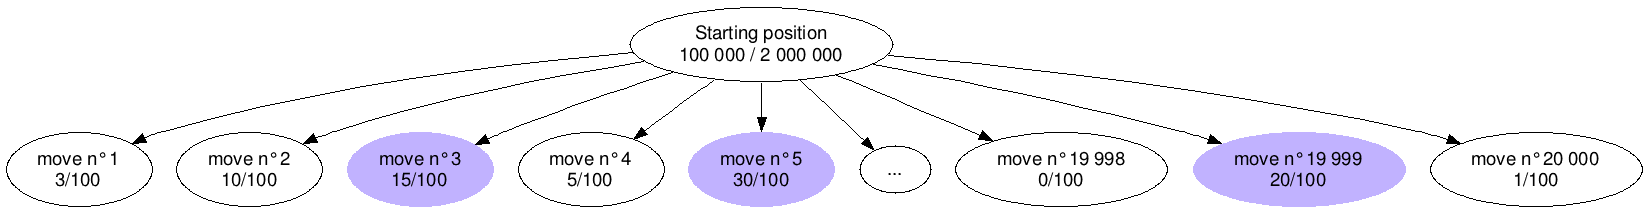
\includegraphics[width=\textwidth]{3Methods/3.2MCTS/img/root.png}
	\caption{\label{fig:roottree}Run random simulations on each childs and select the ones with the highest winrate (Monte Carlo algorithm).}
\end{figure}

\begin{figure}[H]
\centering
	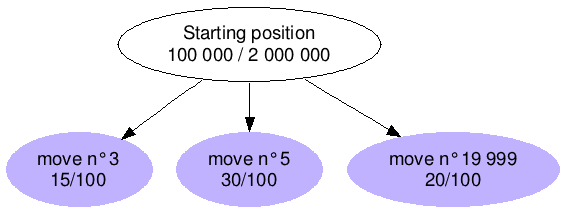
\includegraphics[height=2.5cm]{3Methods/3.2MCTS/img/prune.png}
	\caption{\label{fig:prune}Prune the unselected children.}
\end{figure}

\begin{figure}[H]
\centering
	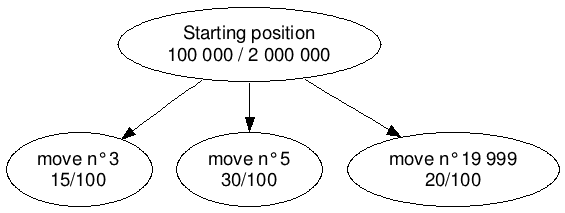
\includegraphics[height=2.5cm]{3Methods/3.2MCTS/img/prune-clean.png}
	\caption{\label{fig:prune-clean}Select the node to expand next (here Move n$^{\circ}$5) using the UCT function.}
\end{figure}

\begin{figure}[H]
\centering
	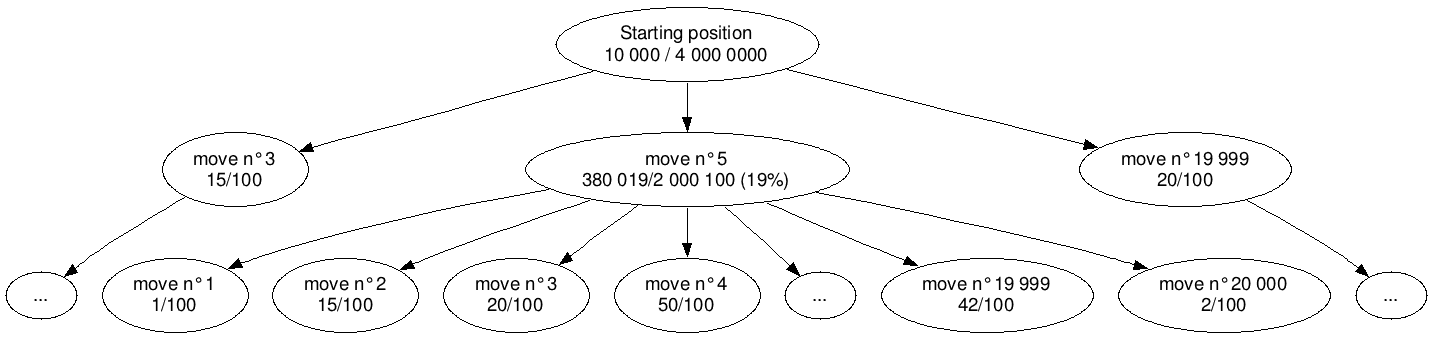
\includegraphics[width=\textwidth]{3Methods/3.2MCTS/img/depth1.png}
	\caption{\label{fig:depth1}Run random simulations on each children and feed back the results to the parents.}
\end{figure}

\begin{figure}[H]
\centering
	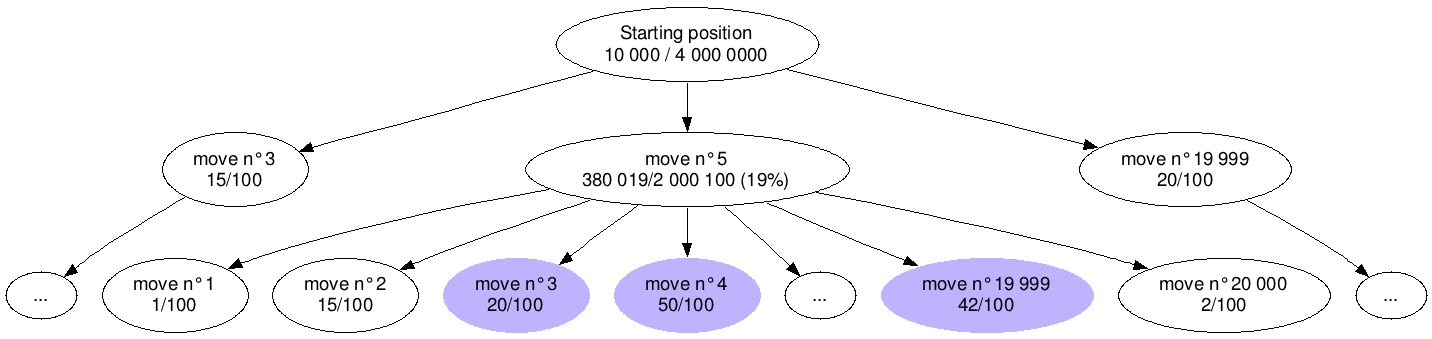
\includegraphics[width=\textwidth]{3Methods/3.2MCTS/img/depth1-select.png}
	\caption{\label{fig:depth1-select}Select the nodes with the highest winrate.}
\end{figure}

\begin{figure}[H]
\centering
	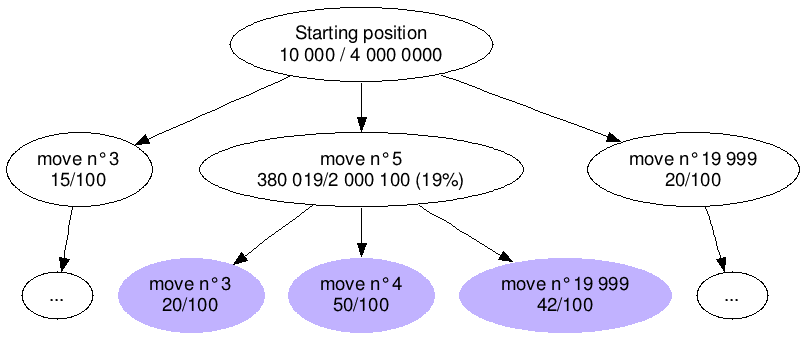
\includegraphics[height=4cm]{3Methods/3.2MCTS/img/depth1-prune.png}
	\caption{\label{fig:depth1-prune}Prune unselected children.}
\end{figure}

Iterate the process until the time limit dedicated to the search is reached and return the move with the highest winrate.